\chapter{Introduction : les 3 enseignements}

\mn{Cours du 20/09/23}


\section{présentation du glossaire}
\paragraph{l'opposition (Dieu / Satan) n'est pas chinoise} Opposition complémentaire. 
voir p. \pageref{DefGlossaire} pour voir les opposées : 

\begin{Ex}[Opposition]
    Voir Yi à li. L'homme de bien doit s'interesser aux questions morales, alors que l'homme pauvre ne va s'intéresser qu'à la richesse.
\end{Ex}.

\begin{Def}[Sanjiao 三教]
    les Trois Enseignements (le confucianisme, le taoïsme et le bouddhisme) 
\end{Def}


\section{le confucianisme}

\begin{Def}[rujiao  儒教]
 sous les Zhou occidentaux, relations familiales. Relations ritualisées.    
\end{Def}


\section{Quelques caractéristiques saillantes de la pensée chinoise}

\begin{singlequote}
    Aucun philosophe occidental ne songerait à nier le rôle de la Grèce dans les origines et les orientations dominantes de nos traditions philosophiques. La claire distinction de l’intelligible et du sensible, de la vérité et de l’opinion, de l’être et du devenir, a été décisive et fondamentale. Or les Chinois n’ont pas admis l’idée d’un domaine propre à la pensée abstraite et au raisonnement logique sur des abstractions. Ils ignorent toute théorie et tout système, et les œuvres de leurs penseurs se présentent le plus souvent comme une suite de notes ou comme des commentaires à des œuvres plus anciennes. Leurs réflexions les plus remarquables sont généralement associées à des préoccupations d’ordre pratique: comment, par exemple, se perfectionner soi-même ou parvenir à l’harmonie sociale?
 
À vrai dire, il n’y a pas en Chine de philosophes de profession. On n’y aurait donc affaire qu’à une forme encore balbutiante de philosophie et tout au plus pourrait-on parler de sagesse.
Et, en effet, il y aurait abus à juger des conceptions chinoises en fonction de nos propres critères, sans admettre qu’ils puissent être remis en cause. Or, c’est à cette remise en cause que peut inciter l’examen d’un certain nombre de thèmes fondamentaux de la pensée chinoise qui forment un ensemble dont la cohérence est manifeste.
\textit{Jacques Gernet, « Introduction à la pensée chinoise », dans Sylvain AUROUX (dir.), La pensée chinoise,
Paris : Quadrige, 2017, p. XXIII.
}

\end{singlequote}

\begin{singlequote}
    Si on devait caractériser d’un mot ce qui fait l’originalité de cette pensée par rapport à nos traditions philosophiques– et même, de façon plus générale, par rapport à nos habitudes mentales–, c’est la notion d’inclusion ou de logique de l’inclusion qui conviendrait le mieux. La pensée chinoise répugne à opposer des contradictoires et à exclure. Ce n’est pas qu’elle ignore le principe de contradiction, dont elle fait usage aussi bien que nous, mais elle ne lui a pas accordé le rôle privilégié que nous lui attribuons. Le thème mythique de la lutte entre natures ennemies (dieux et titans, lumière et ténèbres, Dieu et Satan), ce thème n’est pas chinois. Pour la pensée chinoise, ce sont des opposés complémentaires, non exclusifs les uns des autres, qui forment la trame du monde.\textit{-- Jacques Gernet, ibid., p. XXVI.}
\end{singlequote}


\section{confucianisme - rujiao    }
Confucius : latinisation de Maître Kong, Kongfuzi.  551-479 av. J.-C.


\paragraph{Sous les zhou} la guerre est ritualisée et permet de régler les conflits. 
Mais dans la seconde moitié de cette dynastie, les liens de parenté sont distendus et font d'avantage la guerre pour développer leurs territoires. C'est pendant cette période que Confucius vit et voit les traditionnelles normes s'écrouler.




\paragraph{recueil de poèmes qui fait partie de l'éducation de l'élite, un livre sur les rites...} 5 livres. Forme le noyau de la tradition confucéenne. Etudié jusqu'à début du XX.

\paragraph{débat sur confucius} Pour certains, il a vraiment existé avec une fonction politique, en plus de son enseignement. D'autres chercheurs (américains) pensent qu'il n'a pas existé.

\paragraph{université impériale} on n'enseigne que le Confucianisme. Importanced reso. Les Hans veulent gouverner non par les \textit{lois } mais par les \textit{vertus}. Idéal confucianiste. Les fonctionnaires, quand ils arrivent dans leur poste, la première chose qu'ils font, c'est d'établir une école pour transmettre les vertus.

\paragraph{doctrine officielle sous les Han}{Les Hans, légalisme à l'extérieur, confucianisme à l'intérieur}
les Hans veulent établir un système cohérent de la Foi  : rang de chaque dieux.
 Au IIème siècle avant notre ère (début de la dynastie Han), le confucianisme devint la doctrine officielle de l’État. Sous les Han (202 av. J.-C. – 220 apr. J.-C.), l’État commença à puiser dans la tradition confucéenne pour organiser les rites sacrificiels impériaux afin d’assurer la prospérité de l’empire.
Les réformes rituelles furent achevées au milieu de la dynastie.  
l’une des dimensions de la religiosité du confucianisme
\begin{Synthesis}
    On voit la volonté de contrôler le pouvoir des Hans.
    On pourrait parler d'une religion \textit{civique}, insistant sur les rites sociaux et les vertus (voir religion civique Romaine). 
\end{Synthesis}
\mn{voir cours de christologie et culture, la confrontation avec la \textit{religio} romaine p. \pageref{Def:Religio}.}

\paragraph{une religion ou pas ? } Ce qui rattache à une religion : les rites; Ce qui ne rattache pas à une religion : le \textit{ciel} rattache à la nature et non à Dieu. 

\paragraph{gros travail des philosophes Han} pour organiser les savoirs.

\paragraph{renouveau Song. \textit{le neoconfucianisme}} La dynastie Song (960-1279), grand moment de renouveau du confucianisme sur le plan théorique grâce aux emprunts faits au bouddhisme et au taoïsme  le néoconfucianisme devint la nouvelle idéologie d’État et le restera jusqu’au début du 20ème siècle.
 Floraison et systématisation des rites familiaux


\section{Taoisme}

\begin{Def}[daojiao 道教]
    remonte à Laozi, avec deux textes fondamentaux : 
    \begin{itemize}
        \item le \textit{Daode Jing} : le Livre de la Voie et de la Vertu, IV-III s av JC
        \item le Zhuangzi
    \end{itemize}
\end{Def}

\paragraph{divinisation de Laozi} au 2ème siècle de notre ère, avec l'apparition du taoïsme et de la religion. 

\paragraph{Certains membres de l'aristocratie commencent à lui rendre hommage.}
Les transformations du taoïsme à partir du 3ème siècle . religion acceptée par la haute société. Apparition des premiers monastères taoïstes subventionnés par l’aristocratie.

\paragraph{Les pratiques de Longue Vie}   Ge Hong (283-343). Voir plus loin.


\paragraph{Tang et song} La dynastie Tang (618-907), grande période d’épanouissement du taoïsme.
 Sous la dynastie Song (960-1279), développement de l’alchimie intérieure (neidan  ) par opposition à l’alchimie extérieure (waidan   )

\paragraph{Une notion fondamentale : la voie}
\begin{Def}[dao 道]
    Voie, chemin ; Voie à suivre (en morale, en politique); règle (morale); voie morale; principe (métaphysique) ;      Le Dao : la Voie, vérité ultime ou réalité ultime. La Voie qui ne peut être appréhendée par l’esprit discursif, mais est manifestée ds le devenir naturel des Dix mille êtres. Réalité suprême qui transcende les modalités sensibles et non sensibles de l’être, mais que l’on connaît par l’expérience qu’en donne la pratique de la vertu (德 de).
\end{Def}

\begin{Def}[daode 道德]
    vertu, morale, moralité, bonnes mœurs ; (Philos. chin. – Tao.) la Voie et la vertu / la Voie et sa vertu
\end{Def}
Vérité qui se site au delà de toute différentiation.  Dimension absolue. 


\subsection{Daode jing}
\begin{Def}[Daode jing 道德經]
    Livre de la Voie et de la vertu / Classique de la Voie et de sa vertu  
\end{Def}

Le livre parle de ce que c'est la voie mais aussi de \textit{la pratique} pour l'atteindre ou \textit{y retourner}. On est toujours "dispersé" par l'environnement. Pour retrouver la vérité, il faut diriger son esprit vers l'intérieur.

\paragraph{Une idée de \textit{non-agir}}

dans le sens de non gouvernement de soi. Mais aussi pour la politique, l'empereur ne doit pas trop en faire et laisser les gens faire, car ils connaissent la nature.

\subsection{le Zhuangzi}

Il est plus probable que Zhuangzi ait existé, IVème avant notre ère. Il reprend la notion de la voie, le non-agir et la sérenité. Mais il n'aborde plus la dimension politique.

l'homme peut se transformer.

Le Zhuangzi est plus poétique, parle d'un grand sage qui s'intègre dans la nature, alors que le Daode jing est plus sec ("des proverbes" ?).

\paragraph{Les pratiques de Longue Vie immortalité - alchimie} un des objectifs des Taoistes. A la fin des Hans, des méthodes très concrètes pour les taoistes. \textit{Elixir} très sophistiqué pour vivre l'immortalité (Pb, Or, Mercure). \sn{des empereurs Tang ont avalé cet elixir et en sont morts.}

\begin{Def}[jing 精]
    surchoix, élite ; pur ; fin, subtil, délicat, raffiné. (Philos. chin.) Essence : puissance de vie façonnant et maintenant spécifiquement les êtres. Sans forme mais pourvues de qualités, les essences sont la base des formes corporelles et physiques comme des formes mentales et psychologiques. Sperme. (Tao.) 1. Essence : la forme la plus subtile de la vie. 2. Énergie sexuelle ; force vitale. 3. Éléments liquides et yin du corps. 4. Premier stade de l’œuvre alchimique. 
\end{Def}

\paragraph{Ge Hong. } Comment éviter de perdre l'énergie de l'essence afin de retourner à l'origine de la vie. 

\paragraph{des révoltes paysannes qui ont entrainés la disparition des Han} diffusion du Taoisme. 


\paragraph{5ème siècle : monastère} payé par les aristocrates, intéressés par l'elixir de longue vie. Et ainsi, une religion de paysans touchent l'aristocratie. 

\paragraph{XIII : une image forte, alchimie intérieur} On se rend compte du danger de l'elixir \textit{extérieur}. Le nom des différents métaux devient des symboles. Le feu devient l'esprit. L'eau. A travers la méditation, on arrive à diriger notre énergie pour que les différents éléments (Or, Argent, Mc) qui sont symboliquement dans notre corps, fusionnent. Mettre l'énergie vers le nombril.



\section{Le Bouddhisme - fojiao}

\paragraph{Apparition en Chine au Ier siècle ap. JC}


\begin{itemize}
 \item 	Religion apparue en Inde au 6ème ou 5ème siècle av. J.- C. et introduite en Chine au 1er siècle apr. J.-C., dans la seconde moitié de la dynastie Han.
 \item 	Entre le 3ème et le 6ème siècles, propagation rapide du bouddhisme sur tout le territoire chinois.
 
 \begin{marginfigure}
 \caption{déploiement du grand véhicule}
     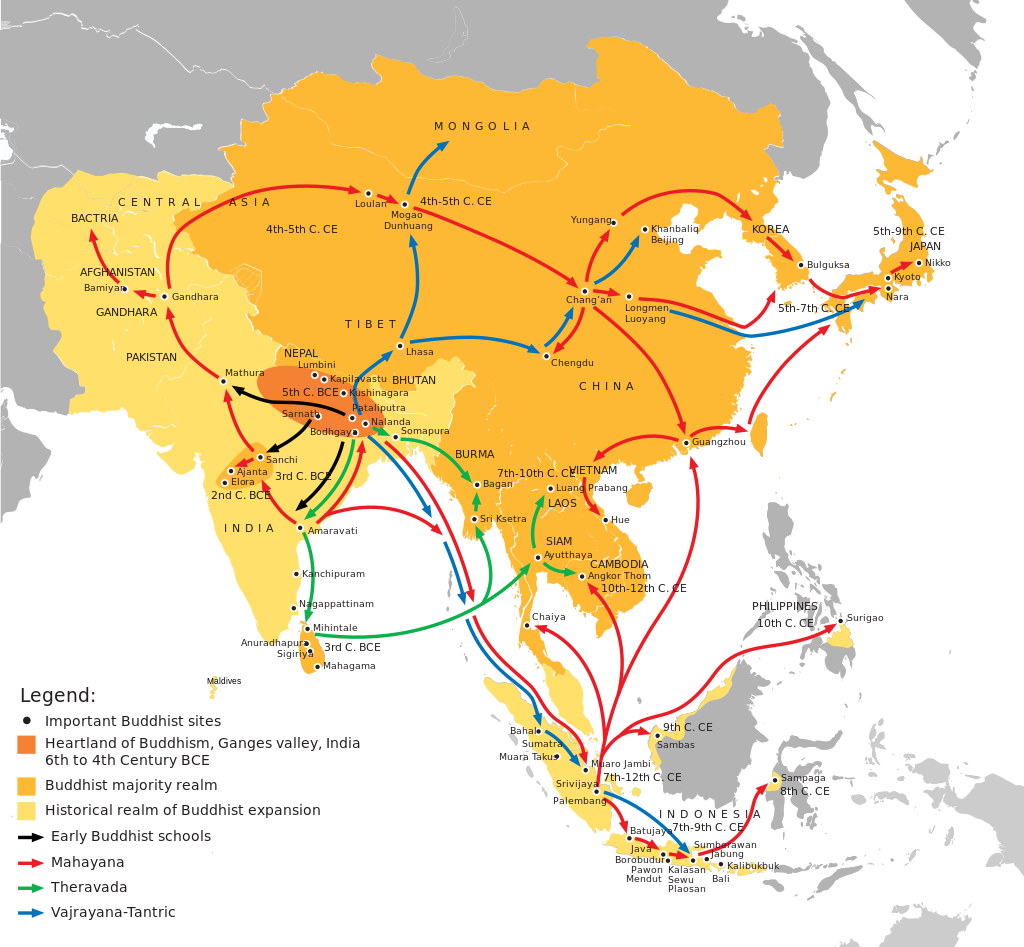
\includegraphics[width=\textwidth]{ConfucianismeTaoismeBouddhismeChinois/Images/Buddhist_Expansion.png}
 \end{marginfigure}
 \begin{Def}[Mahāyāna (Grand véhicule)]
    Plus approfondi que le bouddhisme ancien.   Il conçoit la sainteté non comme un idéal individuel de perfection (arhat), mais comme une carrière visant à entraîner les autres créatures vers le salut.  
\end{Def}
 \item Deux courants du Mahāyāna (Grand véhicule) introduits en Chine poseront les bases pour les écoles bouddhiques chinoises : le Mādhyamaka (la Voie du milieu) et le Vijñanavāda (Rien que
connaissance). Une démarche \textit{plus efficace} pour ses disciples qui voient de façon négative le petit véhicule. 

 \item De la fin du 6ème siècle au 10ème siècle (dynasties Sui et Tang) : formation et développement des écoles bouddhiques proprement chinoises. Le bouddhisme est entièrement sinisé.
écoles les plus importantes: Tiantai (Terrasse céleste), Jingtu (Terre pure), Chan.
\end{itemize}


\section{religions en Chine}
\paragraph{Le problème avec le concept de « religion »:}

\begin{itemize}
    \item  	Le concept occidental moderne de religion:
un système structuré de croyances et de pratiques, séparé de la société, qui organise les fidèles en Église.
    \item  Il n’existe pas en chinois d’équivalent précis du concept occidental moderne de la « religion ».
    \item  	un néologisme adopté du japonais : zongjiao  
    \begin{Def}[zongjiao - 宗教 ]
    Religion au sens moderne, néologisme du japonais  Shūkyō
\end{Def}
    \item  	Ce mot s’impose à l’usage à partir de 1901 dans la langue chinoise.
    \item le problème étant que c'est un mot occidental, on aurait tendance à prendre le christianisme comme référence. Or, c'est différent. 
    
\end{itemize}

\begin{Synthesis}
    Aucun des 3 enseignements chinois n'obligent à l'exclusivité. On est un peu des trois en même temps. 
\end{Synthesis}

 
\subsection{Les Cultes locaux - Religion Populaire}


\begin{Ex}[temple du dieu des Murs et des Fossés]

    \begin{figure}[!h]
        \centering
                \sidecaption{temple du dieu des Murs et des Fossés Shanghai (à gauche) et Xi’an (au milieu et à droite)}
                \includegraphics[width=.4\textwidth]{ConfucianismeTaoismeBouddhismeChinois/Images/TempleDieuMurFosséShanghai.jpg}
    \includegraphics[width=.25\textwidth]{ConfucianismeTaoismeBouddhismeChinois/Images/TempleDieuMurFosséXian.jpg}
        \includegraphics[width=.25\textwidth]{ConfucianismeTaoismeBouddhismeChinois/Images/TempleDieuMurFosséXian2.jpg}

        

        \label{fig:enter-label}
    \end{figure}
    Chenghuang, muraille et fossé, est le nom du dieu protecteur de la ville. Shen signifie dieu. Chenghuangshen est donc le dieu de la ville, des murs et des fossés. couramment mais souvent à tort, puisqu'il suffit d'être hors du territoire pour porter ce nom.

    Dans beaucoup de villes, on peut voir des cultures pour de Dieu des murailles et fossé, sans que celui-ci appartienne à l'un des trois enseignements. Taoisme et Bouddhisme participent à ces rites.
\end{Ex}

\begin{Ex}[temple de la déesse maritime et de la paix]
Là encore, un Dieu qui ne fait pas partie du panthéon taoiste ou bouddhique.
        \begin{figure}[!h]
        \centering
                \sidecaption{temple de la déesse maritime et de la paix - Ville de Tianjin}
                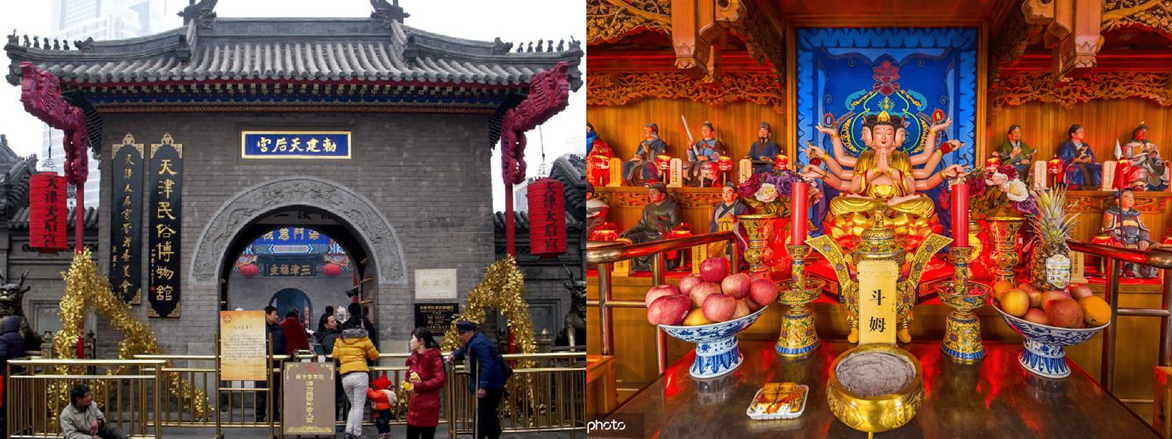
\includegraphics[width=1\textwidth]{ConfucianismeTaoismeBouddhismeChinois/Images/TempleDeesseMaritimeTianjin.png}

        

        \label{fig:enter-label}
    \end{figure}
Là où il y a de l'eau de mer, il y a des Chinois, et là où il y a des Chinois, il y a Mazu.
Connue sous divers noms tels que Tianfei (Dame du palais céleste), Tianhou (Impératrice céleste) ou Tianshang Shengmu (Notre-Dame du Ciel), Mazu est une divinité vénérée par les bateliers, les marins, les voyageurs, les hommes d'affaires et les pêcheurs de toutes les dynasties. Devenue la « Déesse de la mer » au centre des croyances orientales sur le littoral sud-est de la Chine, à l'heure actuelle, des dizaines de milliers de temples lui étant dédiés sont répartis dans 49 pays et régions du monde.
\end{Ex}
\begin{Ex}[Guan Yu ]
général divinisé, les trois enseignements l'utilisent. Il est considéré comme \textit{protecteur de la loi Bouddhique}, ...
        \begin{figure}[!h]
        \centering
                \sidecaption{A gauche et au centre, 
Temple de Guan Yu dans la province du Shanxi, région natale du personnage.
A droite, Statue de Guan Yu dans un temple bouddhique à Hangzhou}
                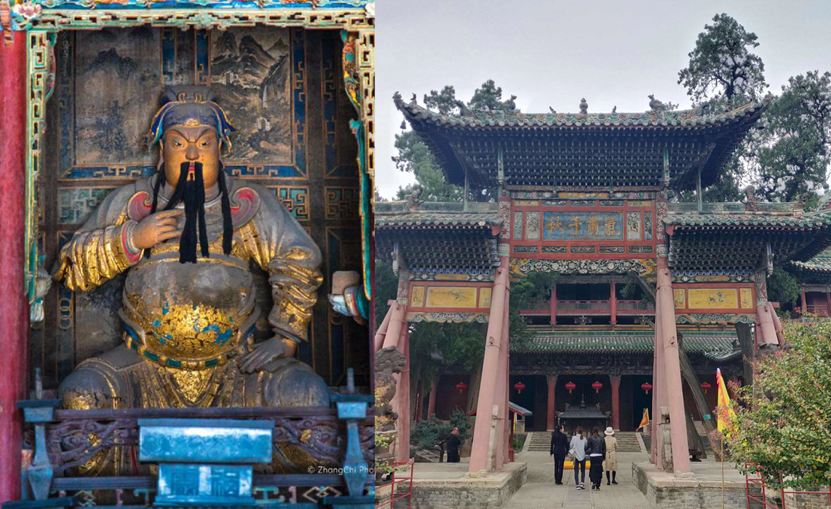
\includegraphics[width=0.6\textwidth]{ConfucianismeTaoismeBouddhismeChinois/Images/TempleGuanYu.png}
                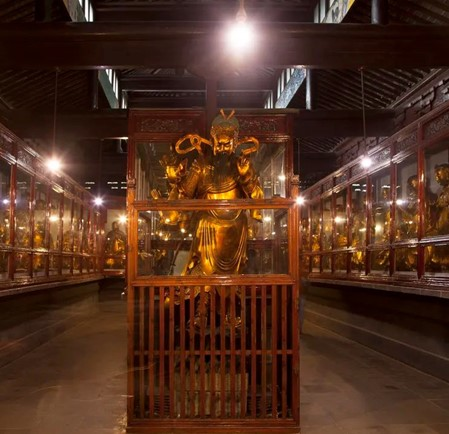
\includegraphics[width=0.35\textwidth]{ConfucianismeTaoismeBouddhismeChinois/Images/StatueGuanYu.jpg}
        

        \label{fig:enter-label}
    \end{figure}
    Guan Yu ou Kouan Yu (chinois simplifié : 关羽 ; chinois traditionnel : 關羽 ; pinyin : guān yǔ), né vers 160-162 et décédé vers octobre 219-220, qui avait pris comme prénom usuel Yunchang1 (chinois simplifié : 云长 ; chinois traditionnel : 雲長 ; pinyin : yún cháng), et qu'on mentionne souvent sous le nom de Guan Gong (chinois traditionnel : 關公, Seigneur Guan), était un général chinois de la fin de la dynastie Han et du début de la période des Trois Royaumes.

Il servit sous les ordres de Liu Bei, le fondateur du royaume de Shu, dont il est le frère d'arme avec Zhang Fei, et aurait été un des cinq « généraux tigres », avec Huang Zhong, Ma Chao, Zhang Fei et Zhao Yun, bien qu’on ignore s’il a effectivement porté ce titre. Réputé de son vivant guerrier invincible, il a été capturé et exécuté, avec son fils Guan Ping par les troupes de Sun Quan, par Lu Meng lors du siège de Fan. Il a été divinisé quelques siècles après sa mort sous le nom de Guanshengdijun (關聖帝君) ou Guandi, « Saint empereur Guan ». Il est toujours vénéré de nos jours en Chine, aussi bien par les taoïstes que par les bouddhistes. Il est particulièrement populaire à Hong-Kong comme dieu de la guerre, des hommes d’affaires et des policiers. On le représente traditionnellement comme un géant à face rouge (symbolisant la loyauté et la droiture) avec une très longue barbe et portant un guandao (une arme d’hast à hampe moyenne de l’époque des Song) qui pesait, selon la légende, plus de 80 jins (environ 40 kg). Il a été immortalisé dans le roman des Trois Royaumes, où il est dépeint comme un guerrier loyal et honorable capable d'exploits surhumains.
\end{Ex}

\begin{Ex}[Temple des lamas Yonghe de Pékin]

On voit des jeunes et on a l'impression qu'ils sont très fervents. Mais sans doctrine, ils viennent pour demander quelque chose. AInsi, dans ce temple Lama Yonghe, on acquiert un bracelet et le voeu est exaucé. Ici, plutôt voeu de  carrière. 
        \begin{figure}[!h]
        \centering
                \caption{Temple des lamas Yonghe de Pékin}
                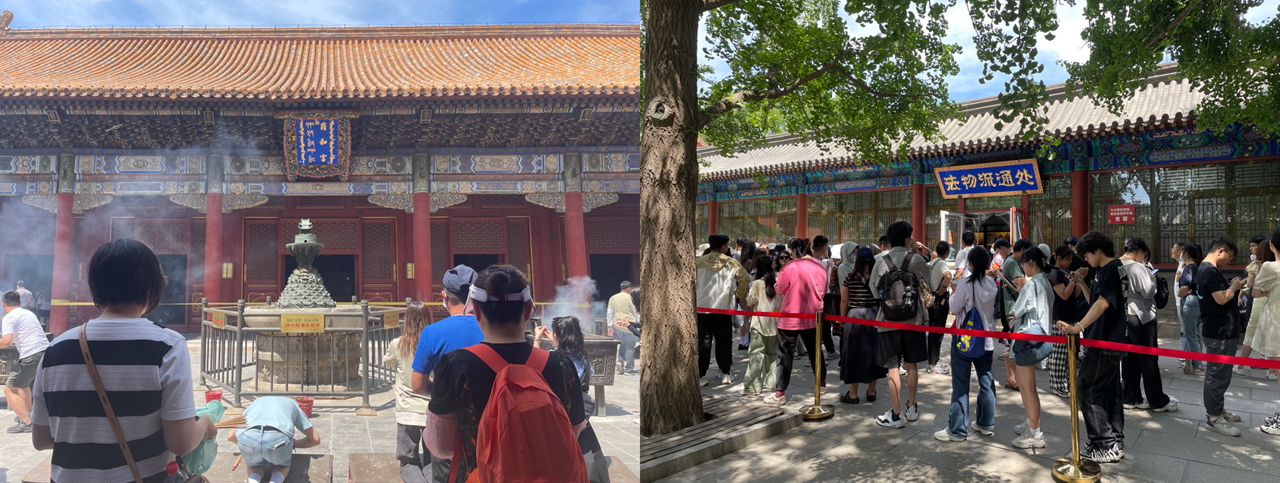
\includegraphics[width=1\textwidth]{ConfucianismeTaoismeBouddhismeChinois/Images/TempleLamaYonghe.png}
            

        \label{fig:enter-label}
    \end{figure}
    Le Temple de Yonghe ou Temple des Lamas ou « Lamaserie Yonghe » ou Yonghe Gong (chinois : 雍和宫 ; pinyin : yōnghé gōng ; litt. « palais de la paix et de l'harmonie ») est un temple du bouddhisme tibétain de Pékin fondé en 1722, sous la dynastie Qing. Le premier bâtiment a été construit en 1694, d'abord pour abriter les eunuques.

Une des statues représente un bodhisattva debout atteignant une hauteur de douze mètres. Différents bâtiments abritent toutes les formes de Bouddha et Bodhisattva typiquement tibétaines. Ce site accueille également des expositions temporaires sur le bouddhisme tibétain.

Les cérémonies religieuses tibétaines y sont toujours pratiquées par des moines tibétains et han.
\end{Ex}

\FloatBarrier
\begin{Def}[ religion chinoise par Vincent Goossaert :]
    \begin{itemize}
        \item 	Un système cohérent, de nature englobante, \textit{non} \textit{exclusive}.
\item 	Elle comprend l’ensemble des formes de pratique religieuse individuelle (méditation, techniques de salut, techniques du corps dont les art martiaux, accès à la connaissance et à la révélation par la transe et l’écriture inspirée) et collective (cultes aux saints locaux, aux ancêtres, rites funéraires)
\item 	Ces pratiques s’inscrivent dans le cadre de la cosmologie chinoise.

    \end{itemize}
\end{Def}
\begin{marginfigure}
\sidecaption{photo de la grand mère du professeur. On voit Mao, derrière un ex-voto pour remercier le Dieu}
      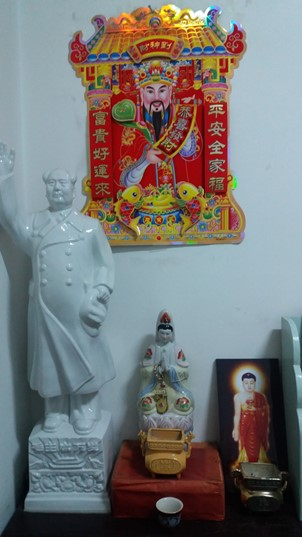
\includegraphics[width=1\textwidth]{ConfucianismeTaoismeBouddhismeChinois/Images/ReligionChine.jpg}
\end{marginfigure}
\begin{Prop}






La religion chinoise existe sans avoir de nom propre, parce qu’elle n’a pas de structure ecclésiale ni d’autorité dogmatique globale.


\end{Prop}

Elle rassemble l’ensemble des formes de la vie religieuses en Chine, à l’exception de certaines religions d’origine étrangère qui, parce qu’elles revendiquent une adhésion exclusive et un monopole de la vérité, n’ont pu s’y intégrer : les trois monothéismes, islam, judaïsme, christianisme. \sn{« Le concept de religion en Chine et l’Occident », Diogène, 2004/1, n°205, p. 11-21}

\section{Le 20ème siècle comme tournant historique}
 

Avant cette époque, la religion chinoise était déjà caractérisée par la diversité, mais elle était structurée autour d’un centre de contrôle : l’État \textbf{politico-religieux.}
\begin{itemize}

    \item  	Cette collusion avec le pouvoir conféra au confucianisme un statut privilégié dans le champ religieux.
    \item le culte confucianisme existait dans le cadre de cet état politico-religieux mais qui a disparu avec la chute de l'empire.
    \item	Face aux cultes locaux nombreux et divers, l’État essaya de distinguer l’orthodoxe de l’hétérodoxe en établissant le registre des  

  \end{itemize}

\paragraph{Hétérodoxie et orthodoxie} ∗ La frontière entre l’orthodoxe et l’hétérodoxe est pourtant assez floue. Quels sacrifices sont reconnus par l’État? C’est une question en constante négociation entre la population et le pouvoir.

\paragraph{après 1912}Après 1912, fin du régime impérial.
Les rituels et les sacrifices confucianistes ont perdu leur place dans la politique.

\paragraph{statut de confucianisme} Quel statut accorder au confucianisme aujourd’hui? Débat toujours en cours
\paragraph{Distinction entre la religion et la superstition.}
Les cinq religions reconnues: catholicisme, protestantisme, islam, bouddhisme, taoïsme.

\begin{itemize}
    \item  	Aujourd’hui: réhabilitation des cultes locaux : la catégorie de
« religion populaire » vient remplacer celle de « superstition » dans les discours académiques.
   \item 	Dans les faits, l’idée de superstition reste ancrée dans l’esprit des chinois sans que celle-ci puisse être définie de manière rigoureuse.
\end{itemize}

\subsection{Importance du Temple}

\paragraph{Vincent GOOSSAERT, Dans les temples de la Chine - critique de Hervieu léger}

L’auteur de ce livre se définit lui-même comme un inlassable déchiffreur d’inscriptions. Les milliers de stèles qu’il a examinées lui ont fourni la matière d’un ouvrage dont le grand intérêt est d’offrir une introduction synthétique à la « religion de la Chine ». De cette religion, l’A. a choisi de traiter dans son unité, sans distinguer entre les « grandes » religions (confucianisme, taoïsme, bouddhisme) et les « petites » traditions, sans distinguer non plus entre les formes populaires de la religiosité et la religion des élites. Car l’unité de cette religion découle de la place centrale qu’y occupe le temple – le bâtiment même – considéré comme le lieu par excellence de la pratique religieuse et de la coexistence entre les différentes traditions établies. Très peu de temples relèvent en effet d’une seule tradition, administrée et défendue par son propre clergé. Dans leur immense majorité, les temples chinois sont des espaces où coexistent et cohabitent, selon de savantes hiérarchies, de multiples divinités grandes ou petites, auxquelles les fidèles rendent un culte. Un culte qui prend physiquement la forme d’un « parcours des offrandes ».

2Pour saisir la logique de cette cohabitation -qui prend à revers les conceptions spontanées que nous avons de la subordination des pratiques cultuelles à des « croyances obligatoires » en principe clairement distinguées comme telles par les fidèles – il faut entrer dans la logique des lieux, et c’est à quoi nous entraîne la « visite guidée » d’un temple proposée par V.G. Il faut également saisir les principes paradoxaux de l’administration des temples par l’État : une administration qui s’étend aux « canonisations » (à l’enregistrement) des divinités autorisées et à l’édiction des canons scripturaux des trois grandes traditions mères, mais qui s’exerce en fait dans des limites extrêmement étroites dans la mesure où prime avant tout le respect de l’équilibre des positions. Dans ce contexte formellement mais faiblement administré, prolifèrent depuis des siècles les fondations les plus diverses, étatiques ou privées, immenses ou minuscules. Ces espaces sont chargés de fonctions multiples : lieux du culte des ancêtres, de l’audience entre le fidèle et la divinité et de l’expression d’une communauté locale, ils peuvent également être cour de justice, théâtre et opéra. V.G. retrace les différentes phases historiques au fil desquelles la Chine est devenue « un pays couvert de temples » : des rites anciens à l’égard des ancêtres à l’arrivée du bouddhisme, de la prolifération des cultes populaires à la mise en place de la doctrine de coexistence entre les trois religions sous la dynastie Tang, de la volonté d’emprise confucianiste sur la scène religieuse au fractionnement local de l’organisation communautaire sous les Ming et les Qing et à la prolifération des sectes populaires. Cette vie religieuse conflictuelle et incontrôlable renforça l’hostilité des élites politiques à l’égard des temples : leur densité maximum (environ 1 million de temples en 1900) est atteinte au moment où s’ouvre l’ère de leur destruction systématique. Il ne reste aujourd’hui en Chine que quelques milliers de temples en activité. À partir de cette mise en perspective historique indispensable, V.G. décline les différents aspects de la vie religieuse, économique et culturelle de ces lieux, faisant apparaître, par-delà la diversité infinie des conditions de fondation et des situations locales, la fonction majeure des temples et de leurs clergés dans la définition et de la redéfinition permanente des rapports entre le public et le privé, dans la production du lien social local, dans la légitimation des pouvoirs et dans l’élaboration des normes de la vie collective. Ce livre, à la fois savant et accessible, sera utile à beaucoup.